\chapter{Poisson Process}
\begin{tcolorbox}
\textbf{Poisson process} is a continuous-time counting stochastic process obtained from a Binomial counting process when its frame size $\Delta$ decreases to 0 while the arrival rate $\lambda$ remains constant. 
\end{tcolorbox}


\begin{itemize}
    \item \textbf{Marginal Distribution}
    $$N(t) \sim Po(\lambda t) \quad t > 0 \quad N(0) = 1$$

    \item \textbf{Transition Probabilities}
    $$
    \mathcal{P}_{m,n+m}(h) = \mathbb{P}[N(t+h) = n+m|N(t)=m] = \begin{cases} 1-\lambda h + o(h) & \mbox{if } n = 0 \\ 
    \lambda h + o(h) & \mbox{if } n = 1\\
    o(h) & \mbox{if } n > 1\\ \end{cases}
    $$

    \item \textbf{Transition Increments}
    \begin{align*}
    \mathcal{P}_{m,n+m}(h) &= \mathbb{P}[N(t+h) = n+m|N(t)=m] \\
    & = \mathbb{P}[N(t+h - t) = n+m - m|N(0)=0]\\
    & = \mathbb{P}[N(h) = n]\\
    & = \sum_{x=0}^n \frac{e^{-\lambda t} (\lambda t)^x}{x!} \text{ used also for }  \mathbb{P}[N(h) \leq n]
    \end{align*}

   \item \textbf{Independent Increments}
   $$(s_1, t_1) \cap (s_2, t_2) = \emptyset \rightarrow N(t_1) - N(s_1) \indep N(t_2) - N(s_2)$$
\end{itemize}

\begin{tcolorbox}
\textbf{Poisson Process}
    \begin{itemize}
        \item \(X(t) = Poisson(\lambda t) \text{ refer to propriety of the Pois with param. } \lambda t\) 
        \item \(T = Exponential(\lambda) \text{ refer to propriety of the Exp with param. } \lambda \)
        \item \(T_k = Gamma(k,\lambda) \text{ refer to propriety of the Gam with params. } \lambda \text{ and } k\)
        \item \(\mathbb{P}[T_k \leq t] = \mathbb{P}[X(t) \geq k]\)
        \item \(\mathbb{P}[T_k > t] = \mathbb{P}[X(t) < k]\)
    \end{itemize}
\end{tcolorbox}

\begin{figure}[h]
\begin{center}
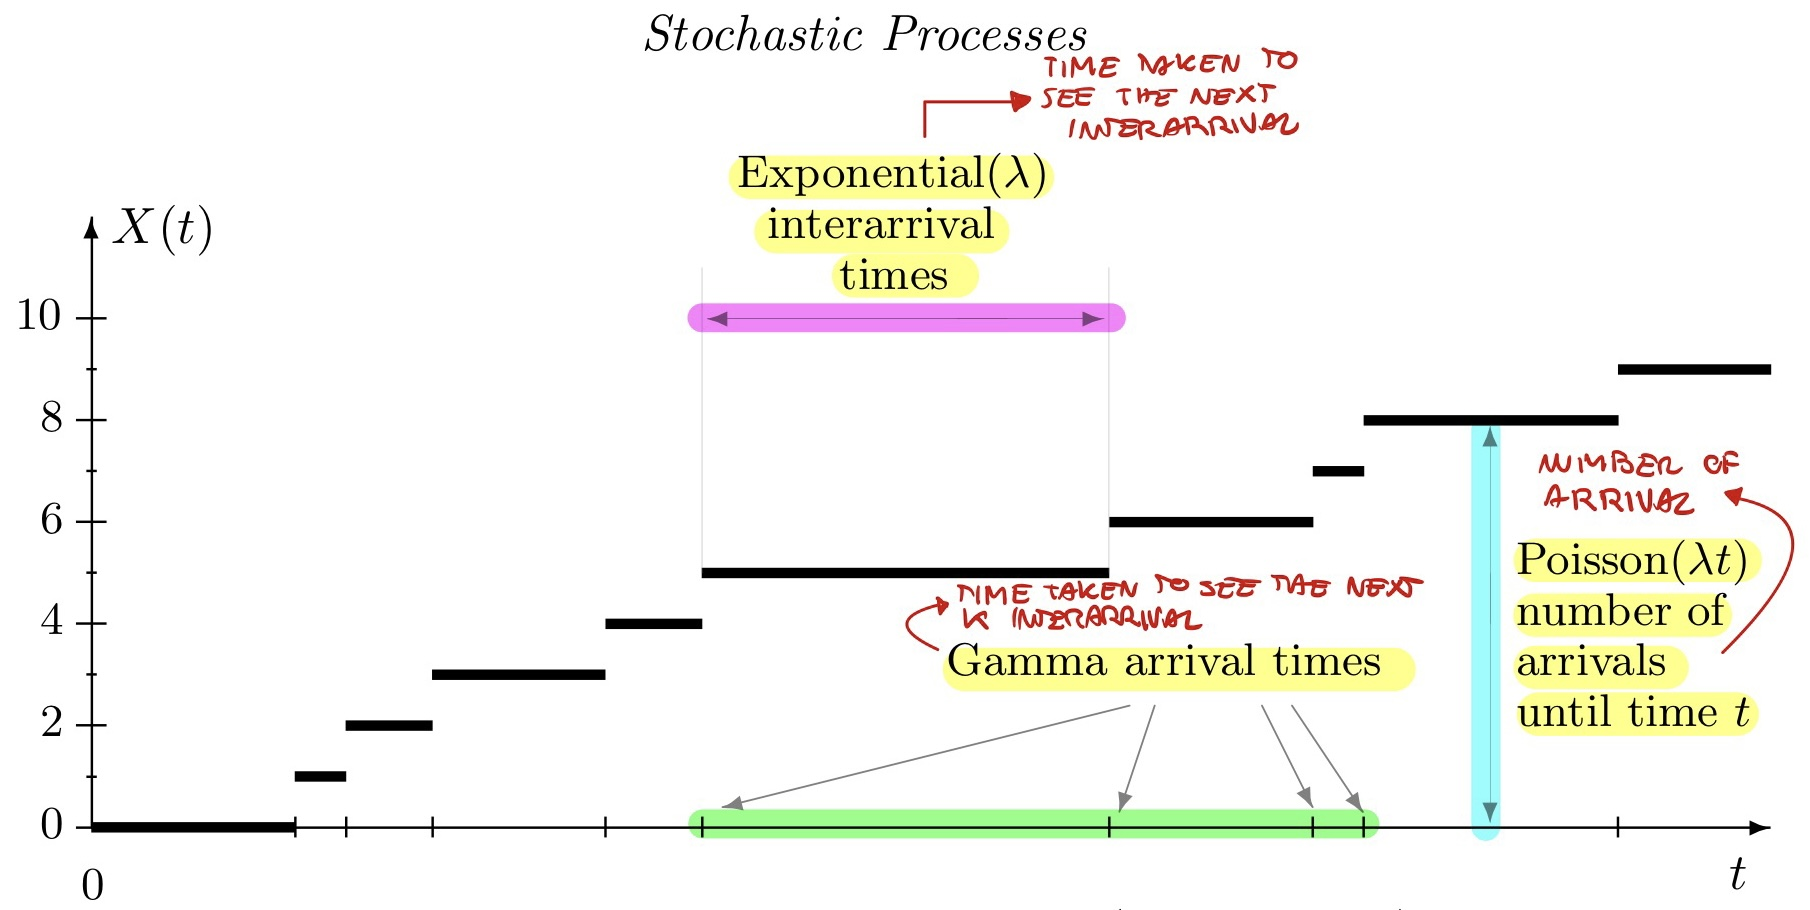
\includegraphics[width=1\linewidth]{images/poisson_process.jpeg}
\end{center}
\end{figure}

\section{Definitions}
\subsection{Definition 1}
A Poisson Process with intensity $\lambda$ is a \textit{Continuous-Time Counting Process} $N=\{N(t): t \geq 0\}$ taking values in $S = \{0,1,2,...\} = \mathbb{N}$ s.t.:
\begin{enumerate}
    \item $N(0) = 0$
    \item \textbf{The increments are independent and stationary} st $N(t+h) - N(t)$ depends only on $h$
    \item $P[N(h) = 1] = \lambda h + o(h)$ and $P[N \geq 2] = o(h)$
\end{enumerate}

\subsection{Definition 2}
A Poisson Process with intensity $\lambda$ is a \textit{Continuous-Time Counting Process} $N=\{N(t): t \geq 0\}$ s.t.
\begin{enumerate}
    \item $N(0) = 0$
    \item For each non overlapping time intervals $(s_1, s_1+t_1]$ and $(s_2, s_2+t_2]$ for $t_1,t_2,s_1,s_2 \geq 0$ the increments $N(s_1+t_1) - N(s_1)$ and $N(s_2+t_2) - N(s_2)$ are \textbf{independent}
    \item $\forall t,s \geq 0$ the \textbf{increment} $N(t+s) - N(s)$ has a \textbf{Poisson} $(\lambda t)$ distribution
\end{enumerate}

\subsection{Definition 3}
A Poisson Process with intensity $\lambda$ is a \textit{Continuous-Time Counting Process} $N=\{N(t): t \geq 0\}$ s.t.
\begin{enumerate}
    \item $N(0) = 0$
    \item Let $T_0 = 0$ and $\forall n \geq 1$ $T_n = inf\{t:N(t) = n\}$ be the n-th arrival time, then the \textbf{nterarrival times} $X_n = T_n - T_{n-1}$ are \textit{iid} \textbf{exponential random variables} with rate $\lambda$
\end{enumerate}

\section{Proprieties}
\subsection{Superposition}
$$N_i \stackrel{\text{iid}}{\sim} PP(\lambda_i) \rightarrow N = \sum_{i=1}^\infty N_i \sim PP(\lambda) \quad \text{where} \quad \lambda = \sum_{i=1}^\infty \lambda_i \text{ must be finite}$$

\subsection{Thinning}
$N \sim PP(\lambda)$ and each arrival assigned to process $N_i$ with probability $p_i$ independently from all others for $p_i \in (0,1)$ such that:
$$\sum_{i=1}^\infty p_i = 1 \quad \quad N_i \stackrel{\text{ind}}{\sim} PP(\lambda \cdot p_i)$$

\subsection{Auto-covariance - $\sigma(s,t) = COV(N(s), N(t))$}
\begin{itemize}
    \item If $s > t$ we split into $[0,s) = [0,t) \cup (t,s]$
    \begin{align*}
    COV(N(t), N(s)) = & COV(N(t), N(t) + N(s) - N(t)))\\
    & COV(N(t),N(t)) + COV(N(t), N(s) - N(t))\\
    & VAR(N(t)) + 0 = \lambda t
    \end{align*}
    \item If $t > s$ we split into $[0,t) = [0,s) \cup (s,t]$
    \begin{align*}
    COV(N(s), N(t)) = & COV(N(s) + N(t) - N(s), N(t)))\\
    & COV(N(s),N(s)) + COV(N(t) - N(s), N(s))\\
    & VAR(N(s)) + 0 = \lambda s
    \end{align*}
\end{itemize}
Thus we obtain that the auto-covariance is equal to 
$$\sigma(s,t) = COV(N(s), N(t)) = \lambda(min\{s,t\})$$

